\documentclass[xcolor=table]{beamer}

\usenavigationsymbolstemplate{}
\setbeamertemplate{footline}[frame number]

\usepackage{graphicx}
\usepackage{hyperref}
\usepackage{tikz}
\usepackage{booktabs}

\title{MAT013 - SAS/R}
\date{2013/12/03}
\author{Vincent Knight + Izabela Komenda}

\begin{document}

\frame{\titlepage}

\frame{\frametitle{SAS}
\begin{center}

\includegraphics[width=6cm]{./Images/SAS.jpg}
\end{center}
}

\frame{\frametitle{R}
\begin{center}

\includegraphics[width=5cm]{./Images/R.pdf}
\end{center}
}

\frame{\frametitle{Users}
\begin{itemize}
\item SAS
    \begin{itemize}
        \item BNP Paribas, Lloyds, \dots
        \item Verison, Vodafone, \dots
        \item Expedia, Photobucket, \dots
    \end{itemize}
\item R
    \begin{itemize}
        \item ANZ, Lloyd's, \dots
        \item Facebook, Google, \dots
        \item Okcupid, New Scientist, \dots
    \end{itemize}
And many more\dots
\end{itemize}
}

\frame{\frametitle{Course Content}
\begin{center}
Taught in parallel:

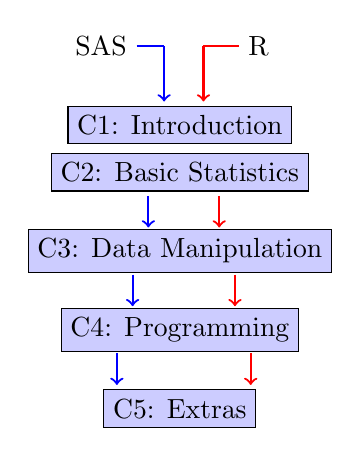
\begin{tikzpicture}
\node (SAS) at (-1, 0) {SAS};
\node (R) at (1, 0) {R};

\draw [blue, thick] (SAS) -- (-.2,0);
\draw [red, thick] (R) -- (.3,0);

\draw [blue, thick, ->] (-.2,0) -- (-.2,-.7);
\draw [red, thick, ->] (.3,0) -- (.3,-.7);

\node [draw, fill=blue!20] (C1) at (0, -1) {C1: Introduction};
\node [draw, fill=blue!20] (C2) at (0, -1.6) {C2: Basic Statistics};

\draw [blue, thick, ->] (-.4,-1.9) -- (-.4,-2.3);
\draw [red, thick, ->] (.5,-1.9) -- (.5,-2.3);

\node [draw, fill=blue!20] (C3) at (0, -2.6) {C3: Data Manipulation};

\draw [blue, thick, ->] (-.6,-2.9) -- (-.6,-3.3);
\draw [red, thick, ->] (.7,-2.9) -- (.7,-3.3);

\node [draw, fill=blue!20] (C4) at (0, -3.6) {C4: Programming};

\draw [blue, thick, ->] (-.8,-3.9) -- (-.8,-4.3);
\draw [red, thick, ->] (.9,-3.9) -- (.9,-4.3);

\node [draw, fill=blue!20] (C5) at (0, -4.6) {C5: Extras};

\end{tikzpicture}
\end{center}
}

\frame{\frametitle{Format}
4 Wednesdays:

\begin{center}
\begin{tabular}{ll}
\toprule
\cellcolor{blue!20}SAS: Class & 0900\\
\cellcolor{blue!20}SAS: Lab &\\
\midrule
Break & \\
\midrule
\cellcolor{red!20}R: Class& \\
\cellcolor{red!20}R: Lab & 1300 \\
\bottomrule
\end{tabular}
\end{center}
\pause

+1 Wednesday
}

\frame{\frametitle{Assessment}
\begin{itemize}
\item Class test: 40\%
\item Group coursework: 30\%
\item Individual coursework: 30\%
\end{itemize}
}

\frame{\frametitle{Learning}
\only<1>{Robert Lee Moore (1882-1972):}
\begin{center}
\only<1>{\textit{``That student is taught the best who is told the least.''}}
\only<2>{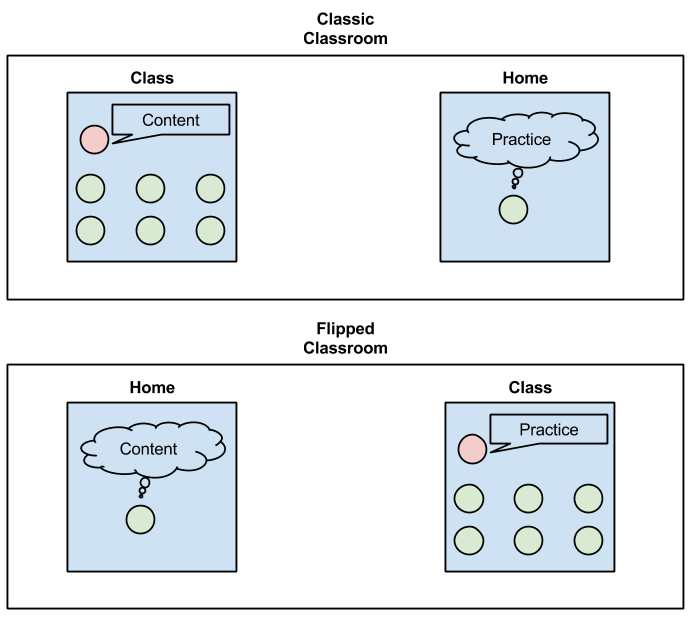
\includegraphics[width=8cm]{./Images/flipped.png}}
\end{center}
}

\frame{\frametitle{Class}
\begin{center}
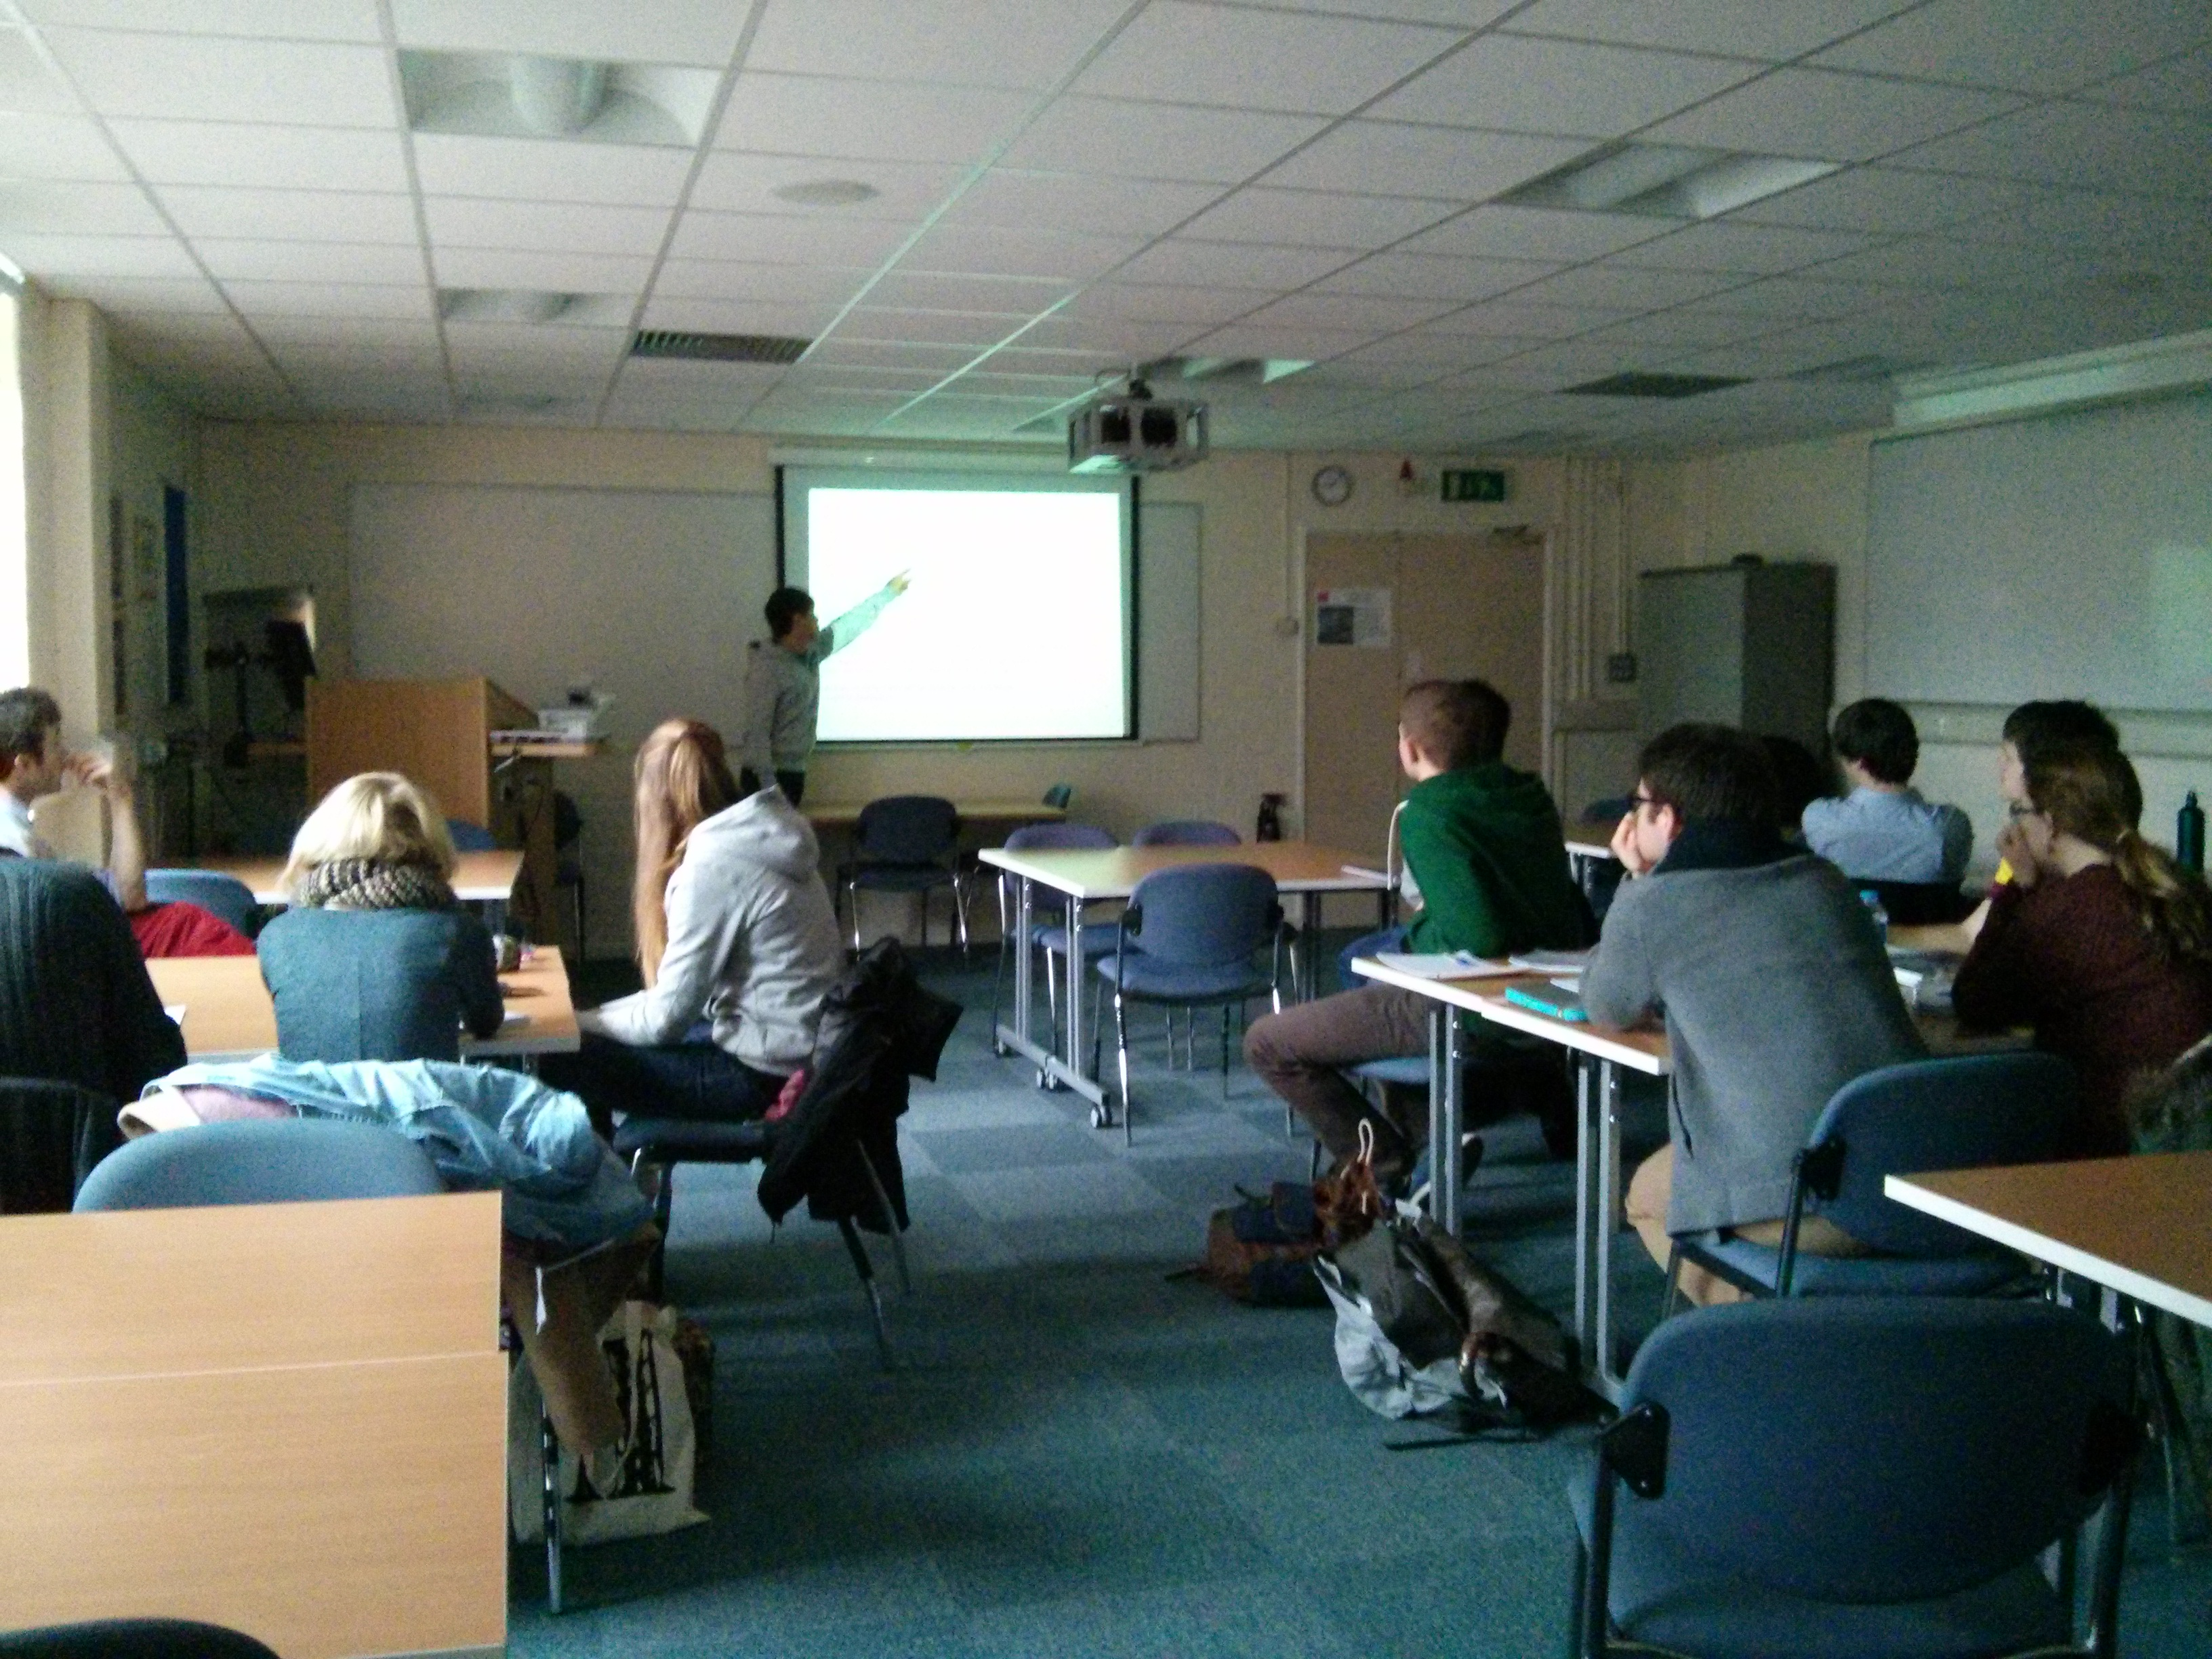
\includegraphics[width=8cm]{./Images/studentpresenting.jpg}
\end{center}
}

\frame{
\begin{center}
\huge{Questions?}\vspace{1cm}

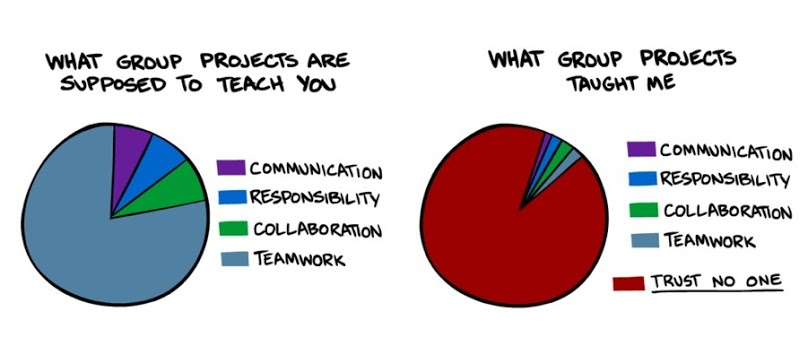
\includegraphics[width=11cm]{./Images/whatgroupprojectsdo.jpg}
\end{center}
}

\end{document}
